\documentclass{article}
\usepackage{floatflt,epsfig}
\usepackage[utf8]{inputenc}
\usepackage[T1]{fontenc}
\usepackage{lipsum}
\usepackage{graphicx}
\usepackage{float}
\usepackage{amsmath}
\usepackage[margin=1in]{geometry}
\usepackage{titlesec}
\usepackage{listings}
\usepackage{xcolor}
\usepackage{tabularx} 
\usepackage{hyperref}
\usepackage{subfigure}
\usepackage{xcolor}

\hypersetup{
    pdfborder = {0 0 0},
}

\definecolor{maroon}{cmyk}{0, 0.87, 0.68, 0.32}
\definecolor{halfgray}{gray}{0.55}
\definecolor{ipython_frame}{RGB}{207, 207, 207}
\definecolor{ipython_bg}{RGB}{247, 247, 247}
\definecolor{ipython_red}{RGB}{186, 33, 33}
\definecolor{ipython_green}{RGB}{0, 128, 0}
\definecolor{ipython_cyan}{RGB}{64, 128, 128}
\definecolor{ipython_purple}{RGB}{170, 34, 255}

\definecolor{outputcellbg}{RGB}{248,248,248}

\lstdefinelanguage{Python}{
    morekeywords={access,and,break,class,continue,def,del,elif,else,except,exec,finally,for,from,global,if,import,in,is,lambda,not,or,pass,print,raise,return,try,while},
    morekeywords=[2]{abs,all,any,basestring,bin,bool,bytearray,callable,chr,classmethod,cmp,compile,complex,delattr,dict,dir,divmod,enumerate,eval,execfile,file,filter,float,format,frozenset,getattr,globals,hasattr,hash,help,hex,id,input,int,isinstance,issubclass,iter,len,list,locals,long,map,max,memoryview,min,next,object,oct,open,ord,pow,property,range,raw_input,reduce,reload,repr,reversed,round,set,setattr,slice,sorted,staticmethod,str,sum,super,tuple,type,unichr,unicode,vars,xrange,zip,apply,buffer,coerce,intern},
    sensitive=true,
    morecomment=[l]\#,
    morestring=[b]',
    morestring=[b]",
    morestring=[s]{'''}{'''},
    morestring=[s]{"""}{"""},
    morestring=[s]{r'}{'},
    morestring=[s]{r"}{"},
    morestring=[s]{r'''}{'''},
    morestring=[s]{r"""}{"""},
    morestring=[s]{u'}{'},
    morestring=[s]{u"}{"},
    morestring=[s]{u'''}{'''},
    morestring=[s]{u"""}{"""},
    literate=
    {á}{{\'a}}1 {é}{{\'e}}1 {í}{{\'i}}1 {ó}{{\'o}}1 {ú}{{\'u}}1
    {Á}{{\'A}}1 {É}{{\'E}}1 {Í}{{\'I}}1 {Ó}{{\'O}}1 {Ú}{{\'U}}1
    {à}{{\`a}}1 {è}{{\`e}}1 {ì}{{\`i}}1 {ò}{{\`o}}1 {ù}{{\`u}}1
    {À}{{\`A}}1 {È}{{\'E}}1 {Ì}{{\`I}}1 {Ò}{{\`O}}1 {Ù}{{\`U}}1
    {ä}{{\"a}}1 {ë}{{\"e}}1 {ï}{{\"i}}1 {ö}{{\"o}}1 {ü}{{\"u}}1
    {Ä}{{\"A}}1 {Ë}{{\"E}}1 {Ï}{{\"I}}1 {Ö}{{\"O}}1 {Ü}{{\"U}}1
    {â}{{\^a}}1 {ê}{{\^e}}1 {î}{{\^i}}1 {ô}{{\^o}}1 {û}{{\^u}}1
    {Â}{{\^A}}1 {Ê}{{\^E}}1 {Î}{{\^I}}1 {Ô}{{\^O}}1 {Û}{{\^U}}1
    {œ}{{\oe}}1 {Œ}{{\OE}}1 {æ}{{\ae}}1 {Æ}{{\AE}}1 {ß}{{\ss}}1
    {ç}{{\c c}}1 {Ç}{{\c C}}1 {ø}{{\o}}1 {å}{{\r a}}1 {Å}{{\r A}}1
    {€}{{\EUR}}1 {£}{{\pounds}}1
    {^}{{{\color{ipython_purple}\^{}}}}1
    {=}{{{\color{ipython_purple}=}}}1
    {+}{{{\color{ipython_purple}+}}}1
    {*}{{{\color{ipython_purple}$^\ast$}}}1
    {/}{{{\color{ipython_purple}/}}}1
    {+=}{{{+=}}}1
    {-=}{{{-=}}}1
    {*=}{{{$^\ast$=}}}1
    {/=}{{{/=}}}1,
    literate=
    *{-}{{{\color{ipython_purple}-}}}1
     {?}{{{\color{ipython_purple}?}}}1,
    identifierstyle=\color{black}\ttfamily,
    commentstyle=\color{ipython_cyan}\ttfamily,
    stringstyle=\color{ipython_red}\ttfamily,
    keepspaces=true,
    showspaces=false,
    showstringspaces=false,
    rulecolor=\color{ipython_frame},
    frame=single,
    frameround={t}{t}{t}{t},
    framexleftmargin=6mm,
    numbers=left,
    numberstyle=\tiny\color{halfgray},
    backgroundcolor=\color{ipython_bg},
    basicstyle=\small,
    keywordstyle=\color{ipython_green}\ttfamily,
}

\lstdefinestyle{Jupyter}{
    sensitive=false,
    keywords={},
    comment=[l]{\#},
    morestring=[b]",
    morestring=[b]',
    morestring=[s]{'''}{'''},
    morestring=[s]{"""}{"""},
    literate=
    {á}{{\'a}}1 {é}{{\'e}}1 {í}{{\'i}}1 {ó}{{\'o}}1 {ú}{{\'u}}1
    {Á}{{\'A}}1 {É}{{\'E}}1 {Í}{{\'I}}1 {Ó}{{\'O}}1 {Ú}{{\'U}}1
    {à}{{\`a}}1 {è}{{\`e}}1 {ì}{{\`i}}1 {ò}{{\`o}}1 {ù}{{\`u}}1
    {À}{{\`A}}1 {È}{{\'E}}1 {Ì}{{\`I}}1 {Ò}{{\`O}}1 {Ù}{{\`U}}1
    {ä}{{\"a}}1 {ë}{{\"e}}1 {ï}{{\"i}}1 {ö}{{\"o}}1 {ü}{{\"u}}1
    {Ä}{{\"A}}1 {Ë}{{\"E}}1 {Ï}{{\"I}}1 {Ö}{{\"O}}1 {Ü}{{\"U}}1
    {â}{{\^a}}1 {ê}{{\^e}}1 {î}{{\^i}}1 {ô}{{\^o}}1 {û}{{\^u}}1
    {Â}{{\^A}}1 {Ê}{{\^E}}1 {Î}{{\^I}}1 {Ô}{{\^O}}1 {Û}{{\^U}}1
    {œ}{{\oe}}1 {Œ}{{\OE}}1 {æ}{{\ae}}1 {Æ}{{\AE}}1 {ß}{{\ss}}1
    {ç}{{\c c}}1 {Ç}{{\c C}}1 {ø}{{\o}}1 {å}{{\r a}}1 {Å}{{\r A}}1
    {€}{{\EUR}}1 {£}{{\pounds}}1,
    keepspaces=true,
    showspaces=false,
    showstringspaces=false,
    upquote=true,
    breaklines=true,
    postbreak=\raisebox{0ex}[0ex][0ex]{\ensuremath{\color{red}\hookrightarrow\space}},
    breakatwhitespace=true,
    tabsize=4,
    basicstyle=\ttfamily\footnotesize,
}

\titleformat{\section}
{\LARGE\bfseries}{\thesection}{1em}{}

\titleformat{\subsection}
{\Large\bfseries}{\thesection}{1em}{}

\begin{document}
    \pagestyle{empty}
    \begin{titlepage}
        \begin{center}
        {{\Large{\textsc{Alma Mater Studiorum - Università di Bologna}}}}
            \rule[0.1cm]{\textwidth}{0.1px}
            \rule[0.5cm]{\textwidth}{0.6px}\\
            {\large{SCUOLA DI SCIENZE \\ Corso di Laurea in Informatica per il Management}}
        \end{center}

        \vspace{90px}

        \begin{center}
            \LARGE Cosmo Catalog Analysis
        \end{center}

        \vspace{100px}
        \par
        \noindent
        \hfill
        \begin{minipage}[t]{0.4\textwidth}\raggedleft
        {\fontsize{12}{13}{}\
            \fontsize{12}{13}{\\ Canghiari Matteo \\ Matricola 1032059 \\ matteo.canghiari@studio.unibo.it}}
        \end{minipage}

        \vspace*{140px}

        \begin{center}
            \large{Statistica Numerica}\\
            \large{Anno Accademico 2023/2024}
        \end{center}
    \end{titlepage}

    \newpage
    \subsection*{Introduzione}
    \large
    \textbf{Cosmo-Catalog-Analysis} è un notebook python realizzato per eseguire un'analisi statistica relativa ad un \href{https://www.kaggle.com/datasets/devendrasingh22/astronomical-data}{\underline{dataset inerente a fenomeni celesti}}. L'obiettivo del progetto consiste nello sviluppo di un'indagine statistica in grado di mettere in luce gli aspetti salienti dell'insieme dei dati. I principali strumenti utilizzati per il caso di studio preso in esame saranno approfonditi nelle sezioni successive, tuttavia è possibile anticipare il contenuto del progetto proposto. \vspace*{7pt}\\
    L'indagine è composta da alcuni passaggi chiave di un'analisi statistica, suddivisi in:
    \begin{itemize}
        \renewcommand{\labelitemi}{-}
        \setlength\parskip{0pt}
        \item \textbf{EDA}, acronimo di Exploratory Data Analysis, il quale costituisce il primo step da affrontare; ottenuto e scelto un dataset sono analizzati i dati contenuti in esso, in maniera tale da evidenziare le informazioni intrinseche e per pianificare lo studio da svolgere
        \item \textbf{Splitting}, fase in cui il dataset è suddiviso in due insiemi, rispettivamente in un train set, utilizzato per l'addestramento del modello di classificazione, e in un test set, impiegato per stabilire la bontà della predizione del modello
        \item \textbf{Regressione lineare}, in cui è stato condotto un problema supervisionato legato alla predizione di una variabile di output y di tipo numerico; lo studio è stato realizzato tra coppie di variabili fortemente correlate, sia positivamente che negativamente
        \item \textbf{Addestramento del modello}, passaggio essenziale affinché i modelli di classificazione, pertanto legati alla predizione di una variabile di output y di tipo categorico, possano stabilire i parametri che minimizzano la funzione di loss
        \item \textbf{Valutazione delle performance}, addestrati i modelli e definiti i parametri associati, lo step successivo prevede lo studio delle performance associate a ciascun algoritmo. La valutazione della bontà del modello avviene attraverso lo studio dei risultati successivi alla fase di predizione 
        \item \textbf{Studio statistico dei risultati}, fase in cui sono impiegate tecniche sia di statistica descrittiva che inferenziale; in particolare per un K fissato, sono state ripetute le fasi di addestramento e di testing per ciascun modello di classificazione, in maniera tale da ottenere uno storico delle metriche valutative associate
    \end{itemize}
    Concludendo, il dataset scelto rivela alcuni aspetti caratteristici dei fenomeni celesti, composto da tutti i domini chiave per l'esplorazione del cosmo. Di seguito, sono riportate brevi descrizioni dei domini trattati, in cui si evidenzia: \vspace*{7pt}\\
    \begin{tabularx}{\textwidth}{|c|X|X|}
        \hline
        1. & \textbf{Temperature} & Informazioni termiche della stella \\
        \hline
        2. & \textbf{Luminosity} & Brillantezza/luminosità della stella \\
        \hline
        3. & \textbf{Radius} & Dimensione spaziale della stella \\
        \hline
        4. & \textbf{Magnitude} & Luce intrinseca della stella \\
        \hline
        5. & \textbf{Star type} & Tipologia della stella \\
        \hline
        6. & \textbf{Star color} & Colore visibile della stella \\
        \hline
        7. & \textbf{Spectral Class} & Classe spettrale della stella \\
        \hline
    \end{tabularx}

    \newpage
    \subsection*{EDA}
    Come riportato dall'introduzione, la prima fase, per un qualsiasi progetto legato ad una indagine statistica, prevede l'analisi dei dati contenuti all'interno del dataset. Un dataset è una tabella di \textit{osservazioni}, in cui le colonne rappresentano le \textit{features}, mentre le righe rappresentano le differenti entità; dal punto di vista matematico un dataset è una matrice di dimensione \textit{$N \times $d}. \vspace*{7pt}\\
    Il dataset scelto ha una dimensione pari a \textit{$240 \times $7}, rispettivamente il numero di righe e di colonne. Le features si contraddistinguono in domini \textit{numerici} e \textit{categorici}, come riportato nella tabella seguente. \vspace*{7pt}\\
    \begin{tabularx}{\textwidth}{|c|X|X|}
        \hline
        1. & \textbf{Temperature} & int64 \\
        \hline
        2. & \textbf{Luminosity} & float64 \\
        \hline
        3. & \textbf{Radius} & float64 \\
        \hline
        4. & \textbf{Magnitude} & float64 \\
        \hline
        5. & \textbf{Star type} & int64 \\
        \hline
        6. & \textbf{Star color} & object \\
        \hline
        7. & \textbf{Spectral Class} & object \\
        \hline
    \end{tabularx} \vspace*{7pt}\\
    Nonostante la colonna \textbf{Star type} sia di tipo numerico non è plausibile un suo impiego all'interno di indagini statistiche, poichè utilizzata principalmente per categorizzare le differenti entità della matrice. \vspace*{7pt}\\
    Il dataset non possiede alcun \textit{dato mancante}, generalmente definito come \textit{NaN}, dato che la sua dimensione non varia successivamente all'eliminazione di osservazioni mancanti. Inoltre, è stato eseguito un rapido controllo relativo alle variabili categoriche; spesso il loro utilizzo avviene per distinguere le moltiplici entità secondo caratteristiche comuni, introducendo delle vere e proprie classi.    
    \begin{lstlisting}[language=Python]
classes = df["Spectral Class"]
_dict = df["Spectral Class"].value_counts().to_dict()

print(_dict)
    \end{lstlisting}
    \begin{lstlisting}[style=Jupyter]
Out: {'M': 111, 'B': 46, 'O': 40, 'A': 19, 'F': 17, 'K': 6, 'G': 1}
    \end{lstlisting}
    Come da snippet di codice precedente, il risultato ottenuto esprime una certa proponderanza di determinate \textit{classi}. A causa di tale sbilanciamento, una caratteristica simile potrebbe causare differenti problematiche associate alla predizione di modelli di classificazione, in questa circostanza è necessario accertarsi che lo splitting del dataset racchiudi ogni possibile associazione tra le differenti features, in modo tale che non si abbiano ripercussioni inerenti alla bontà dei modelli di classificazione. \vspace*{7pt}\\
    Una volta completata l'analisi delle variabili categoriche, il controllo consecutivo è ricaduto sulle variabili numeriche, approfondendo in questo modo la comprensione dei dati. Sono state condotte tutte le tipologie di \textit{indagini}, \textit{univariate}, \textit{bivariate} piuttosto che \textit{multivariate}, ognuna delle quali caratterizzata dai propri strumenti grafici. I principali strumenti grafici impiegati per evidenziare le proprietà statistiche dei vari domini possono essere suddivisi in:
     \begin{itemize}
        \renewcommand{\labelitemi}{-}
        \setlength\parskip{0pt}
        \item \textbf{Boxplot}, strumento grafico usato per visualizzare la distribuzione di una variabile numerica, osservare i quartili ed identificare eventuali valori anomali, detti outlier
        \item \textbf{Istogramma}, strumento grafico per esaminare la distribuzione dei dati e le frequenze corrispondenti, raggrupate in intervalli definiti
        \item \textbf{Grafico a dispersione}, strumento visivo per osservare la relazione tra due variabili numeriche, in cui ogni punto rappresenta un'osservazione del dataset, avente coordinate pari ai valori delle due variabili
        \item \textbf{Matrice di correlazione}, matrice quadrata di dimensione pari al numero di variabili in input impiegate, ogni elemento che compone la matrice corrisponde al grado di correlazione tra due variabili, propriamente denominato \textit{coefficente di correlazione}
    \end{itemize}
    A tal proposito, è interessante osservare la relazione catturata dal \textit{grafico a dispersione} tra le features \textit{Temperature} e \textit{Luminosity}.
    \begin{center}
        \fbox{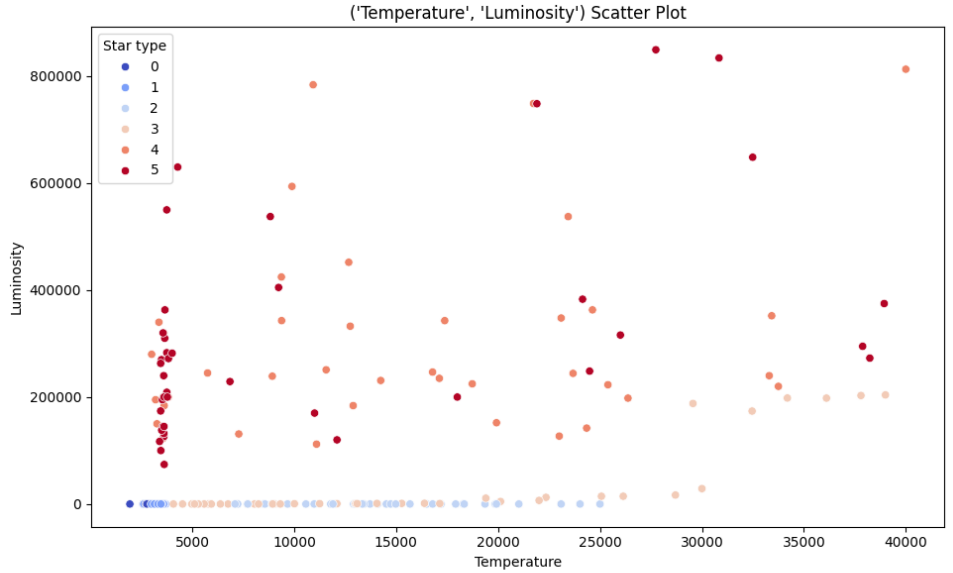
\includegraphics[width=.9\textwidth]{img/img1.png}}
    \end{center}
    Il grafico a dispersione riportato rappresenta un \textit{diagramma di Hertzsprung-Russell}, in quanto mostra la distribuzione dei corpi celesti in base alla loro temperatura e luminosità. Sebbene queste due grandezze fisiche dipendano strettamente da caratteristiche intrinseche della stella, come età, composizione chimica e massa, è evidente una suddivisione stratificata: nella parte inferiore si trovano le stelle più fredde e meno luminose, al centro quelle di temperatura e luminosità intermedie, mentre in alto sono collocate le stelle più calde e brillanti. \vspace*{7pt}\\
    Ultimo passaggio, seppur fondamentale, riguarda l'analisi di valori anomali, detti \textit{outliers}. Un outlier rappresenta un osservazione che si discosta significativamente rispetto ai valori contenuti all'interno della feature presa in considerazione. Una delle tecniche principali per valutare se un dato è un valore anomalo avviene tramite la definizione di un \textit{range interquartile}, ottenuto tramite la differenza tra il terzo e il primo \textit{quartile}. In semplici termini, il range esprime una certa variabilità in cui i dati possono essere considerati validi; se oltrepassato il limite, inferiore oppure superiore, l'osservazione potrebbere rappresentare potenzialmente un valore anomolo.
    \begin{lstlisting}[language=Python]
def define_outliers(df: pd.DataFrame) -> tuple[Dict[str, int], pd.DataFrame]:
    _df = df.select_dtypes(include="number").copy()

    q1 = _df.quantile(0.25)
    q3 = _df.quantile(0.75)

    iqr = q3 - q1
    lower_bound = q1 - 1.5 * iqr
    upper_bound = q3 + 1.5 * iqr

    dict_outliers = {column.strip(): 0 for column in _df.columns}

    for column in _df.columns[1:]:
        for i in range(len(_df[column])):
            if _df.iloc[i][column] > upper_bound[column]:
                _df.iloc[i][column] = upper_bound[column]
                dict_outliers[column] += 1

            if _df.iloc[i][column] < lower_bound[column]:
                _df.iloc[i][column] = lower_bound[column]
                dict_outliers[column] += 1

    return (dict_outliers, _df)
    \end{lstlisting}
    \begin{lstlisting}[style=Jupyter]
Out: {'Temperature': 0, 'Luminosity': 12, 'Radius': 40, 'Absolute magnitude': 0, 'Star type': 0}
    \end{lstlisting}
    
    \newpage
    \subsection*{Regressione lineare}
    I modelli di \textit{regressione lineare} sono implementati qualora il tipo della variabile di output è numerico. Formalmente, in statistica la regressione lineare permette di costruire un modello attraverso cui predire i valori di una variabile dipendente, \textit{Y}, dati i valori di una o più variabili indipendenti, \textit{X}. \vspace*{7pt}\\
    A partire dai risultati ottenuti dalla \textit{matrice di correlazione}, sono state scelti alcuni domini caratterizzati da un \textit{coefficente di correlazione r} positivo, ossia maggiore di 0. Pertanto, il coefficente esprime il grado di dipendenza tra due features. 
    \begin{center}
        \fbox{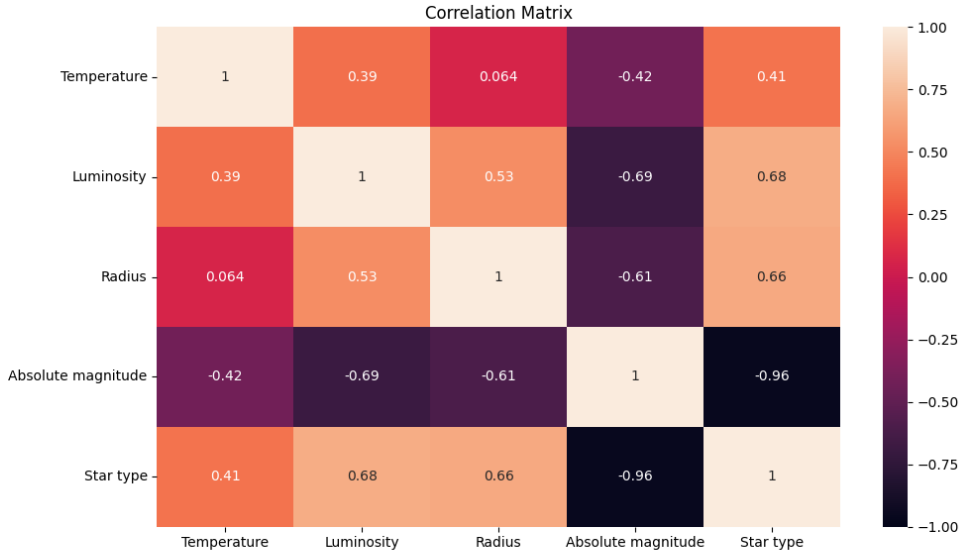
\includegraphics[width=.9\textwidth]{img/img2.png}}
    \end{center}
    L'immagine propone la matrice di correlazione dei domini del dataset di carattere numerico; la colonna \textit{Star type}, nonostante esprima una correlazione positiva nei confronti della maggior parte delle features che contraddistingue l'insieme di dati, non è stata impiegata per realizzare indagini statistiche, poichè è utilizzata principalmente per categorizzare le molteplici entità. A tal proposito, qualsiasi associazione rispetto al dominio \textit{Absolute magnitude} presenta una dipendenza negativa. Questa caratteristica evidenzia un andamento inversamente proporzionale del dominio in esame rispetto agli altri. In particolare, all'aumentare dei valori della variabile \textit{Absolute magnitude}, i dati delle altre colonne tenderanno a diminuire. \vspace*{7pt}\\
    \begin{lstlisting}[language=Python]
X_label = "Radius" 
y_label = "Luminosity"

X = _df[[X_label]]
y = _df[y_label]

univariate_linear_regression(X_label, y_label, X, y)
    \end{lstlisting}
    \begin{lstlisting}[style=Jupyter]
Out: 
In ordine: 
 - m: [182.67977484] 
 - q: 63864.43153126554 
 - R^2: 0.27721880798570075
    \end{lstlisting}
    Lo snippet invoca il metodo indicato per eseguire una regressione lineare univariata, dato che la variabile di input coincide con un solo carattere del dataset. La funzione provvede, in completa autonomia, al calcolo computazionale degli \textit{stimatori} dell'\textit{equazione lineare}, quali \textit{coefficente angolare} ed \textit{intercetta}, mostrando i grafici relativi.
    \begin{center}
        \fbox{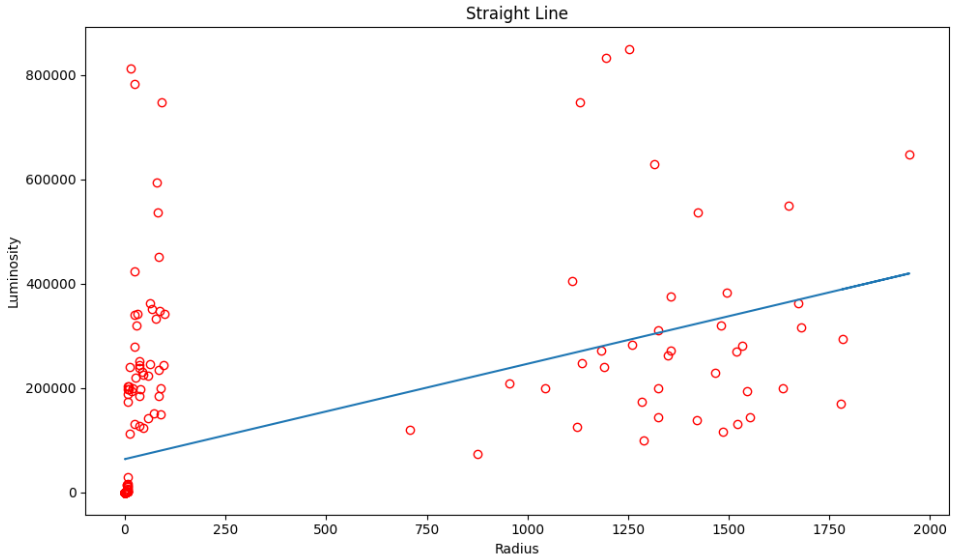
\includegraphics[width=.9\textwidth]{img/img3.png}}
    \end{center}
    A livello visivo, i punti dovrebbero disporsi lungo la retta di equazione
    \begin{center}
        $y=182.68x + 63864.432$ 
    \end{center}
    secondo una certa omogeneità, affinché sia possibile affermare l'accuratezza dell'algoritmo di regressione lineare. Tuttavia, come riportato dall'immagine soprastante, le coppie $(x,y)$ tendono ad uniformarsi in due insiemi suddivisi, testimoniando uno scarso rendimento da parte del modello. Il quadro delineato evidenzia le difficoltà nell'utilizzo di una funzione lineare capace di generare predizioni valide per la variabile di output designata. \vspace*{7pt}\\
    La retta della regressione lineare rappresenta una semplificazione della realtà. Ciò implica che alcune caratteristiche del modello non possano emergere dalla raffigurazione geometrica; proprio per questa principale ragione è necessario implementare un'\textit{analisi dei residui}. I residui costituiscono l'\textit{errore di previsione} del modello di regressione, ottenuti mediante la differenza dei valori esatti rispetto ai valori predetti. La bontà del modello si muove di pari passo alla distribuzione dei residui. Uno score elevato della retta testimonia una distribuzione in cui circa la media è nulla, $\mu=0$, e la varianza, $\sigma^2$, è costante, in modo tale che ciascuna predizione abbia sempre lo stesso grado di variabilità. 
    \begin{center}
        \fbox{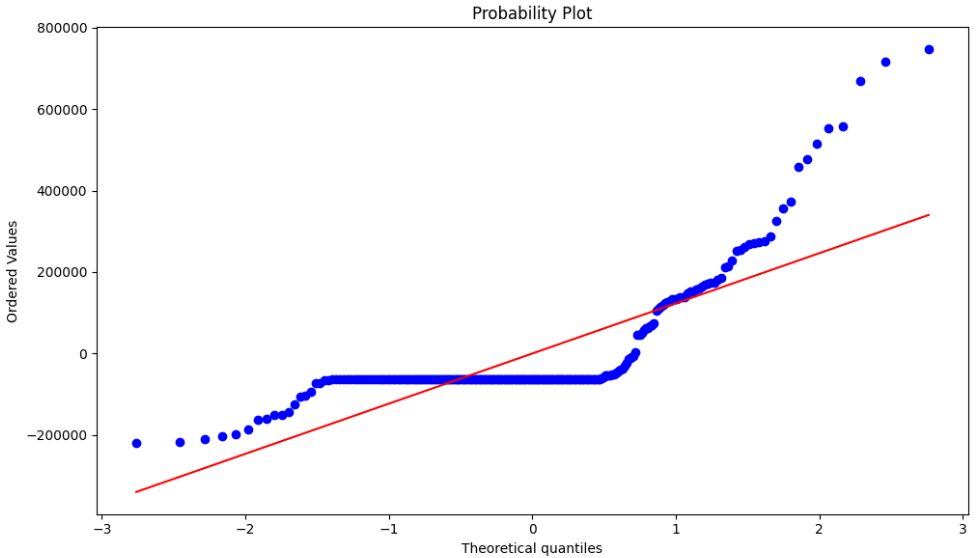
\includegraphics[width=.9\textwidth]{img/img4.png}}
    \end{center}
    Il grafico definisce un \textit{QQ-Plot}, ossia una raffigurazione dei quantili di una distribuzione. Il suo scopo principale consiste nel confrontare la distribuzione di una variabile osservata, in questa circostanza i \textit{residui} del modello di regressione lineare, con la distribuzione della \textit{normale}. Se le due distribuzioni presentano un andamento simile, i punti $(x,y)$ dovrebbero allinearsi lungo alla retta. Pertanto, se i punti si discostano significativamente dalla retta, ciò indica che i residui non seguono una distribuzione normale. Quest'ultimo inciso valorizza la scarsa bontà del modello di regressione lineare implementato, data la notevole discrepanza, suggerendo la necessità di modelli alternativi più adatti alle osservazioni del dataset. 

    \newpage
    \subsection*{Addestramento del modello - Valutazione delle performance}
    Gli algoritmi di classificazione, come la \textit{regressione logistica} e le \textit{Support Vector Machines}, sono implementati qualora la variabile di output è di tipo categorico. In questo caso, la variabile di output potrà assumere soltanto un numero finito di valori, detti \textit{classi}. \vspace*{7pt}\\
    All'interno del progetto è stata attuata una conversione numerica di tali features, affinché i dati contenuti al loro interno fossero manipolabili dai modelli di classificazione.
    \begin{lstlisting}[language=Python]
encoder = preprocessing.LabelEncoder()
df_category = df.select_dtypes(include=["object", "category"])

print("In ordine:", end="\n")
for column in df_category.columns:
    _set = union_categorical_field(column, df)
    values = encoder.fit_transform([item for item in _set])
    _dict = {key: int(value) for key, value in zip(_set, values)}

    print(f"- Dominio \033[1m{column}\033[0m del dataset convertito in 
          {_dict}", end="\n")

    df[column] = df_category[column].map(_dict)
    \end{lstlisting}
    \begin{lstlisting}[style=Jupyter]
Out:
In ordine:
- Dominio Star color del dataset convertito in {'White': 3, 'Red': 2, 'Blue-White': 1, 'Yellow-White': 4, 'Blue': 0}
- Dominio Spectral Class del dataset convertito in {'F': 2, 'A': 0, 'G': 3, 'M': 5, 'K': 4, 'O': 6, 'B': 1}
    \end{lstlisting}
    Successivamente allo snippet di codice dedito alla conversione numerica di colonne categoriche, è stata sviluppata la logica necessaria per usufruire dei modelli di classificazione. \vspace*{7pt}\\
    La regressione logistica è un \textit{classificatore lineare}, utilizzato qualora la variabile dipendente sia di natura categorica. L'obiettivo del modello è di stabilire la probabilità che un'osservazione, appartenente al dataset, possa generare una \textit{classe} della variabile dipendente.
    \begin{lstlisting}[language=Python]
def logistic_regression(X_train, X_test, y_train, y_test):
    try:
        X_train = preprocessing.MinMaxScaler().fit_transform(X_train)
        X_test = preprocessing.MinMaxScaler().fit_transform(X_test)

        model = LogisticRegression(max_iter=100, multi_class="multinomial") 
                .fit(X_train, y_train)

        y_pred = model.predict(X_test)
        accuracy = round(metrics.accuracy_score(y_test, y_pred)*100, 2)
        
        print(f"Accuratezza del modello di regressione logistica: {accuracy}")
    except Exception:
        print("I dataset inviati non rispettano i vincoli di dimensione")        
    \end{lstlisting}
    A livello implementativo è possibile evidenziare due aspetti sostanziali, quali:
    \begin{itemize}
        \renewcommand{\labelitemi}{-}
        \setlength\parskip{0pt}
        \item \textbf{MinMaxScaler}, classe della libreria \textit{preprocessing} di \textit{sklearn}, utilizzata per normalizzare le variabili di input del modello di classificazione. La normalizzazione dei dati avviene affinché le features del dataset caratterizzate da scale differenti non influenzino il modello durante la fase di addestramento, evitando che l'algoritmo sia fondato su predeterminati bias
        \item \textbf{Parametri} della regressione logistica, in cui sono stati definiti il \textit{numero  di iterazioni} e la \textit{tipologia} del modello. Brevemente, \textit{max\_iter} indica il numero massimo di iterazioni che il modello può eseguire per garantire la convergenza della \textit{funzione sigmoide} rispetto alla variabile dipendente, mentre \textit{multi\_class} determina la modalità predittiva dell'algoritmo, tenendo conto della numerosità di classi associabili alla variabile di output
    \end{itemize}
    Conclusa la computazione del metodo, viene mostrata l'\textit{accuratezza} del modello di regressione logistica confrontando i valori predetti rispetti ai dati esatti.
        \begin{lstlisting}[style=Jupyter]
Out:
Accuratezza del modello di regressione logistica: 90.282
    \end{lstlisting}
    Tipicamente, le Support Vector Machines sono implementate qualora il dataset non sia \textit{linearmente separabile}, ossia non esiste alcuna retta o iperpiano separatore in grado di suddividere nettamente le osservazioni della matrice. L'idea alla base dell'algoritmo SVM consiste nella semplificazione del dataset, mediante una certa funzione detta \textit{kernel function}, affinché l'insieme di dati sia successivamente classificabile secondo \textit{modelli SVC}, acronimo di Support Vector Classifier. \vspace*{7pt}\\
    La bontà del modello dipende da due fattori principali, suddivisi in:
    \begin{itemize}
        \renewcommand{\labelitemi}{-}
        \setlength\parskip{0pt}
        \item \textbf{Kernel function}, semplifica e rende il dataset linearmente separabile. In tale ambito, non sono più impiegate rette oppure iperpiani separatori, ma sono introdotte \textit{curve separatrici}, la cui forma è dettata dalla scelta della funzione nucleo
        \item \textbf{Iperparametri}, rappresentano i parametri associati al classificatore, come il \textit{costo} per funzioni lineari, il \textit{grado} dell'esponente per funzioni polinomiali, piuttosto che la \textit{varianza} per funzioni esponenziali
    \end{itemize}
    \begin{lstlisting}[language=Python]
def support_vector_machines(X_train, X_test, y_train, y_test):
    try:
        plt.figure(figsize=(20, 6))

        X_train = preprocessing.MinMaxScaler().fit_transform(X_train)
        X_test = preprocessing.MinMaxScaler().fit_transform(X_test)

        linear_model = svm.SVC(kernel="linear", C=1).fit(X_train, y_train)
        cf_matrix_linear = evaluate_kernel("Lineare", X_test, y_test, linear_model)

        plt.subplot(1, 3, 1)
        plt.title("Linear Confusion Matrix")
        plt.xlabel("True Values")
        plt.ylabel("Predicted Values")
        sns.heatmap(cf_matrix_linear, annot=True, cmap="Reds")

        poly_model = svm.SVC(kernel="poly", degree=3).fit(X_train, y_train)
        cf_matrix_poly = evaluate_kernel("Polinomiale", X_test, y_test, poly_model)

        # Poly Confusion Matrix ...

        rbf_model = svm.SVC(kernel="rbf").fit(X_train, y_train)
        cf_matrix_rbf = evaluate_kernel("Esponenziale", X_test, y_test, rbf_model)

        # Rbf Confusione Matrix ...

        plt.tight_layout()
        plt.show()
    except Exception as e:
        print("I dataset inviati non rispettano i vincoli di dimensione")
    \end{lstlisting}
    Al termine della computazione, sono mostrati il \textit{misclassification ratio}, l'\textit{accuratezza} e la \textit{matrice di confusione} per ciascun modello. Il misclassification ratio è una metrica che esprime la percentuale totale dei punti mal classificati dal predittore; da cui, mediante la formula $$Acc=1-MR(S),$$ è calcolata l'accuratezza, la quale manifesta la bontà del modello predittivo, nonostante non sia effettivamente una metrica.
    \begin{lstlisting}[language=Python]
def evaluate_kernel(type_model, X_test, y_true, model) -> metrics:

    y_pred = model.predict(X_test)

    MR = np.mean(y_pred != y_true)
    accuracy = 1 - MR

    print(f"{type_model}: \n - Misclassification ratio: {round(MR*100, 2)} \n 
    - Accuratezza del modello: {round(accuracy*100, 2)} \n")
    
    return metrics.confusion_matrix(y_true, y_pred)
    \end{lstlisting}
    \begin{lstlisting}[style=Jupyter]
Lineare: 
 - Misclassification ratio: 23.61 
 - Accuratezza del modello: 76.39 

Polinomiale: 
 - Misclassification ratio: 5.56 
 - Accuratezza del modello: 94.44 

Esponenziale: 
 - Misclassification ratio: 5.56 
 - Accuratezza del modello: 94.44 
    \end{lstlisting}
    
    \newpage
    \subsection*{Studio statistico dei risultati}
    Una sola esecuzione dei modelli, ottenuti tramite la Support Vector Machines, non è sufficiente per valutare la bontà degli algoritmi di classificazione, data l'aleatorietà dei dati utilizzati. Per tale ragione, sono state ripetute le fasi di addestramento e di testing per un numero intero K fissato. \vspace{7pt}\\
    L'obiettivo prevede di osservare l'andamento di un modello di classificazione introducendo la \textit{cross-validation}; la convalida incrociata, cosiddetta \textit{k-fold}, consiste nella suddivisione del train set in n parti di equivalente numerosità e, a ogni passo, si esclude iterativamente una sezione alla volta tentando di predirla con i gruppi di dati restanti, al fine di verificare la bontà del modello predittivo, evitando l'\textit{overfit}. Inoltre, ad ogni iterazione è introdotto un certo grado di casualità durante la fase di \textit{splitting} del dataset, in maniera tale che l'addestramento del modello avvenga sempre per suddivisioni differenti dell'insieme di dati.
    \begin{lstlisting}[language=Python]
def evaluate_model(K: int, df: pd.DataFrame, _svm: svm.SVC) -> List[int]:
    print("Accuratezza del modello in ordine:", end="\n")

    accuracies = []
    for i in range(K):
        tuple_dataframes = split_dataframe(randomness=i, 
                                           y_field="Spectral Class", df=df)

        X_train = tuple_dataframes[0]
        X_test = tuple_dataframes[1]

        y_train = tuple_dataframes[2]
        y_test = tuple_dataframes[3]

        model = _svm.fit(X_train, y_train)

        y_pred = model.predict(X_test)

        scores = cross_val_score(_svm, X_train, y_train, scoring="accuracy", 
                        cv=KFold(n_splits=i+1, shuffle=True, random_state=20+2*i))
        mean_accuracy = round(scores.mean()*100, 2) 

        recall = metrics.recall_score(y_test, y_pred, average="weighted",
                                      zero_division=0)
        mean_recall = round(np.mean(recall)*100, 2)
        
        precision = metrics.precision_score(y_test, y_pred, average="weighted", 
                                            zero_division=0)
        mean_precision = round(np.mean(precision)*100, 2)

        print(f"- Step {i+1}: \n\t - Precisione: {mean_precision} \n\t
        - Sensitivita': {mean_recall} \n\t- Accuratezza: {mean_accuracy}", end="\n")
        
        accuracies.append(mean_accuracy)

    return accuracies
    \end{lstlisting}
    \begin{lstlisting}[style=Jupyter]
Accuratezza del modello in ordine:
- Step 1:
	- Precisione: 84.3
	- Sensitività: 84.72
	- Accuratezza: 82.73
- Step 2:
	- ...
	- ...
	- ...
- ...
- Step 10:
	- Precisione: 86.08
	- Sensitività: 86.11
	- Accuratezza: 87.56

L'accuratezza media del modello linear risulta: 85.79
    \end{lstlisting}
    Il risultato evidenzia alcune metriche ottenute dal modello di classificazione secondo la \textit{kernel function} di tipo \textit{lineare}. Ad ogni iterazione del ciclo è riportata la \textit{precisione}, la \textit{sensitività} e l'\textit{accuratezza} dell'algoritmo rispetto alla variabile di output y predetta. Al termine della funzione, è restituita la lista delle accuratezze estrapolate per ciascuna computazione. \vspace*{7pt}\\
    Dalla lista è poi calcolata la \textit{media} delle accuratezze, affinché sia definito un \textit{intervallo di confidenza}.
    Similmente ai \textit{quartili}, gli intervalli di confidenza esprimono un range di variabilità in cui ci si aspetta di inviduare un certo parametro; è necessario affermare che tale tecnica non indica la probabilità, in questa casistica, che la media delle accuretezze sia all'interno di tale intervallo, ma, semplicemente, stabilisce un limite inferiore e superiore in cui dovrebbe collocarsi la metrica presa in esame.
    \begin{lstlisting}[language=Python]
def define_confidence_interval(_list):
    try:
        if check_types_list(float, _list):
            n = len(_list)

            std_accuracy = np.std(_list)
            mean_accuracy = np.mean(_list)

            confidence_interval = stats.t.interval(0.95, n-1, 
                                    loc=np.mean(_list), scale=stats.sem(_list))

            print(f"L'intervallo di confidenza con livello di confidenza alpha=0.05
            risulta: [{confidence_interval[0]}, {confidence_interval[1]}]")
        else: 
            raise Exception
    except Exception:
        print("La lista in input deve contenere solamente valori numerici")
    \end{lstlisting}
    \begin{lstlisting}[style=Jupyter]
L'intervallo di confidenza con livello di confidenza alpha=0.05 risulta: [84.40196998984591, 87.1780300101541]
    \end{lstlisting}
\end{document}